\documentclass{beamer}
\usetheme{Boadilla}
\usepackage{essay-def}
\usepackage{bm}
\usepackage{amsfonts}
\usepackage{amssymb}
\usepackage{amsmath}
\usepackage{amsthm}
\usepackage{comment}
\usepackage{subcaption}
\usepackage{geometry}
\newcommand{\JX}[1]{{\color{red}{$^{\text{JX}}$[#1]}}}
\geometry{left=1cm,right=1cm}
    \title[Model Reduction]{Model reduction: past and present}
\author[ZJX]{Jiaxi Zhao}
\date{23th Oct, 2024}
\begin{document}
\par \setlength{\parindent}{2em}

\begin{frame}
\titlepage

\end{frame}

\begin{frame}{Part I: Existing methods}
	\begin{itemize}
		\item \textbf{Classical methods:}
		\item * Balanced Proper Orthogonal Decomposition (POD)
		\item * Galerkin projection
		\item * Discrete empirical interpolation method (DEIM)
		\item * Koopman operator inspired methods
		\item * Tensor-based methods
		\item \textbf{Modern methods:}
		\item * Nonlinear ROM
		\item * Non-intrusive ROM via operator inference
		\item * Temporal coarsening
	\end{itemize}
\end{frame}


\begin{frame}{Words at the beginning}
	We will focus on \textbf{scientific} time series modeling. Model reduction is related to lots of other terminologies such as 
	modal analysis, reduced-order modeling, etc.

	The key feature of time series modeling:
	\begin{itemize}
		\item * Stability issue
		\item * Extrapolation or interpolation?
	\end{itemize}
	\begin{equation*}
		\begin{aligned}
			& \mfX_1 \rightarrow \mfX_2 \rightarrow \cdots \mfX_n,		\\
			& t_1 \rightarrow \mfX_{t_1}, t_2 \rightarrow \mfX_{t_2}, \cdots
		\end{aligned}
	\end{equation*}
\end{frame}

\begin{frame}{Reduced-order modeling: Past}
	\begin{itemize}
		\item * Balanced Proper Orthogonal Decomposition (POD)
		\item * Galerkin projection
		\item * Discrete empirical interpolation method (DEIM)
		\item * Koopman operator inspired methods
		\item * Tensor-based methods\footnotemark
	\end{itemize}
	\footnotetext{Benner, Peter, et al., eds. Model reduction and approximation: theory and algorithms. Society for Industrial and Applied Mathematics, 2017.}
\end{frame}

\begin{frame}{Modal analysis: POD}
		\begin{figure}[ht]
			\centering
			\centerline{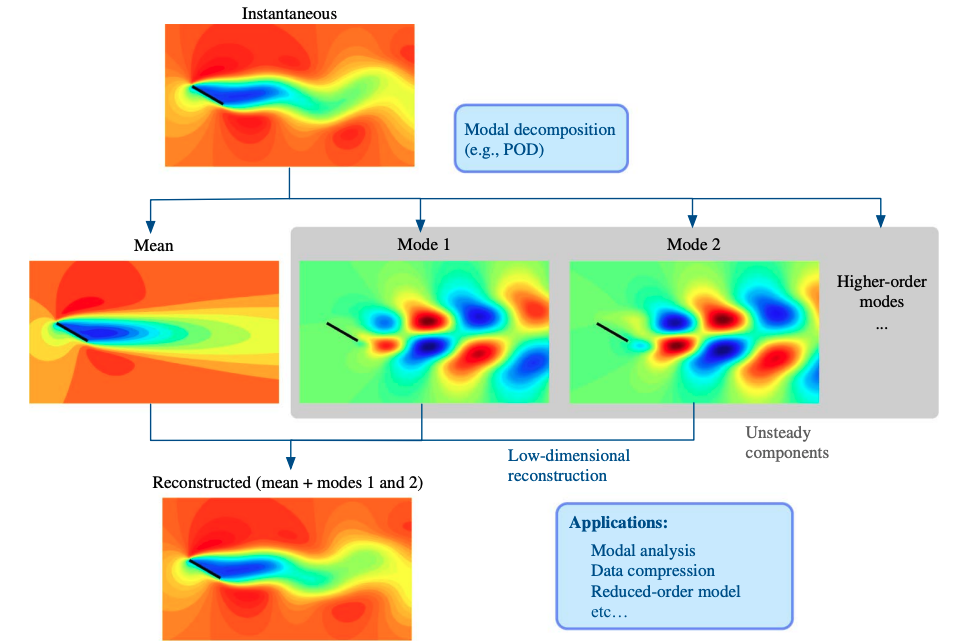
\includegraphics[width=.8\linewidth]{fig/POD.png}}
			\caption{Modal decomposition of two-dimensional incompressible flow over a flat-plate wing $Re=100, \alpha=30$. This example shows
			complex nonlinear separated flow being well represented by only two POD modes and the mean flowfield. Visualized are the streamwise velocity profiles.\footnotemark}
	\end{figure}
	\JX{What do these POD mean physically?}
		\footnotetext{Taira, Kunihiko, et al. "Modal analysis of fluid flows: An overview." Aiaa Journal 55.12 (2017): 4013-4041.}
\end{frame}

\begin{frame}{Balanced Transformation}
	Let us consider the following control system
	\begin{equation*}
		\frac{d}{dt}\mfx(t) = A\mfx(t) + B\mfu(t), \quad \mfy(t) = C\mfx(t).
	\end{equation*}
	The key observation is that any invertible transformation $\wtd \mfx = V\mfx$ will result in
	an equivalent system with different POD basis. For this system, the controllability and observability Grammians are defined as
	\begin{equation*}
		W_c = \int_0^{\infty} e^{At}BB^T e^{A^Tt}dt, \quad W_o = \int_0^{\infty} e^{A^Tt}C^TC e^{At}dt.
	\end{equation*}
	Balanced transformation $V$ is chosen so that the $W_c, W_o$ are diagonal and equal.
	\footnotemark
	\footnotetext{Willcox, Karen, and Jaime Peraire. "Balanced model reduction via the proper orthogonal decomposition." AIAA journal 40.11 (2002): 2323-2330.}
\end{frame}

\begin{frame}{Balanced POD}
	Under the transformation $V$, two Grammians will transform according to
	\begin{equation*}
		\wtd W_c = V^{-1}W_cV^{-T}, \quad \wtd W_o = V^{T}W_oV.
	\end{equation*}
	Then their product transforms as 
	\begin{equation*}
		\wtd W_cW_o = V^{-1}W_cW_oV.
	\end{equation*}
\end{frame}

\begin{frame}{Projection-based ROM}
	We consider two types of problem as follows:
	\begin{equation*}
		\begin{aligned}
			\frac{d}{dt}\mfx(t) & = A\mfx(t) + N(\mfx(t)),\\
			0 & = A_{\mu}\mfx(\mu) + N_{\mu}(\mfx(\mu)), \quad \mfx \in \mbR^{n\times n}.
		\end{aligned}
	\end{equation*}
	In both systems, $N(\cdot)$ represents the nonlinearity. Given any reduced basis functions of order $k$, 
	orthogonal projection operator onto this basis is denoted as $V_k$ with reduced system
	\begin{equation*}
		\begin{aligned}
			\frac{d}{dt}\wtd\mfx(t) & = V_k^T A V_k\wtd\mfx(t) + V_k^T N(V_k\wtd\mfx(t)),\\
			0 & = V_k^T A_{\mu} V_k\wtd\mfx(\mu) + V_k^T N_{\mu}(V_k\wtd\mfx(\mu)), \quad \wtd\mfx \in \mbR^{k\times n}.
		\end{aligned}
	\end{equation*}
\end{frame}

\begin{frame}{DEIM}
	The nonlinear term still remains huge amount of computation:
	\begin{equation*}
		V_k^T N(V_k\wtd\mfx(t)), \quad \wtd J_N(\mfx(\mu)) = V_k^T J_F(V_k\wtd\mfx(\mu))V_k.
	\end{equation*}
	The idea is to project this nonlinear term further onto a low-dimensional subspace spanned by $\lbb \mfu_0, \mfu_1, \cdots, \mfu_m \rbb$
	which is obtained by applying POD to the nonlinear snapshots obtained from the original full-order system.
	\begin{equation*}
		N(V_k\wtd\mfx(t)) = \mfU c(t).
	\end{equation*}
\end{frame}

\begin{frame}{Interpolation method}
	\footnotemark
	\footnotetext{Amsallem, David, and Charbel Farhat. "Interpolation method for adapting reduced-order models and application to aeroelasticity." AIAA journal 46.7 (2008): 1803-1813.
	}
\end{frame}

\begin{frame}{Difficulties of model reduction}
	\begin{itemize}
		\item * Nonlinearity, e.g. convection
		\item * Transient modeling and unsteady, especially for long time prediction and turbulence
	\end{itemize}
\end{frame}

\begin{frame}{Draw-back of linear-subspace ROM}
	In particular, linear-subspace ROMs can be expected to produce
	low-dimensional models with high accuracy\footnotemark only if the problem admits a fast decaying Kolmogorov n-width
	(e.g., diffusion-dominated problems). 
	\begin{equation*}
		d_n(\mcM) := \inf_{\mcS_n}\sup_f\inf_{g\in\mcS_n}\|f-g\|.	
	\end{equation*}
	Unfortunately, many problems of interest exhibit a slowly decaying
	Kolmogorov n-width (e.g., advection-dominated problems).
	\footnotetext{Binev, Peter, et al. "Convergence rates for greedy algorithms in reduced basis methods." SIAM journal on mathematical analysis 43.3 (2011): 1457-1472.}
\end{frame}

\begin{frame}{Koopman operator}
	Methods related to the Koopman operator are related to the dynamics of the operator,
	which is also approximated via a linear dynamics 
	\begin{itemize}
		\item * Extended Dynamical Model Decomposition (EDMD)
		\item * EDMD-DL 
		\item * parametric Koopman
	\end{itemize}
\end{frame}

\begin{frame}{ROM: Present}
	\begin{itemize}
		\item * Nonlinear ROM
		\item * Non-intrusive ROM via operator inference
		\item * Temporal coarsening
	\end{itemize}
\end{frame}

\begin{frame}{Nonlinear trial manifold: learn the reduced basis}
	Nonlinear trial manifold\footnotemark
	\begin{equation*}
		\wtd \mfx(t;\mu)= \mfx_{ref}(\mu) + g(\wht \mfx(t;\mu)),
	\end{equation*}
	where $\mfx_{ref}(\mu)$ denotes the parametrized reference state specified according to the initial condition and $g:\mbR^p \rightarrow \mbR^n$
	denotes the nonlinear parameterization function refered to as \textit{decoder}.	The reduced dynamics can be obtained via chain rule:
	\begin{equation*}
		\frac{d}{dt}\wtd \mfx(t;\mu) = J_g(\wht \mfx(t;\mu))\frac{d}{dt}\wht \mfx(t;\mu).
	\end{equation*}
	\footnotetext{Lee, Kookjin, and Kevin T. Carlberg. "Model reduction of dynamical systems on nonlinear manifolds using deep convolutional autoencoders." Journal of Computational Physics 404 (2020): 108973.}
\end{frame}

\begin{frame}{Time-continuous residual minimization}
	The model can be written using the residue function
	\begin{equation*}
		\mfr(\mfv, \mfx, t, \mu) =  \mfv - f(\mfx, t, \mu).
	\end{equation*}
	Based on this, we can define the equation for the reduced model as 
	\begin{equation*}
		\frac{d}{dt}\wht \mfx(t;\mu) = \arg\min_{\mfv\in\mbR^p}\norml \mfr(J_g(\wht \mfx(t;\mu))\mfv, \mfx_{ref}(\mu) + g(\wht \mfx(t;\mu)), t, \mu) \normr
	\end{equation*}
	Based on this, the truncation error analysis of the ROM can also be performed using approximation theory of the function spaces.
\end{frame}

\begin{frame}{Operator inference: Learn the reduced operator}
	
\end{frame}

\begin{frame}{Temporal coarsening}
	\begin{figure}[ht]
		\centering
		\centerline{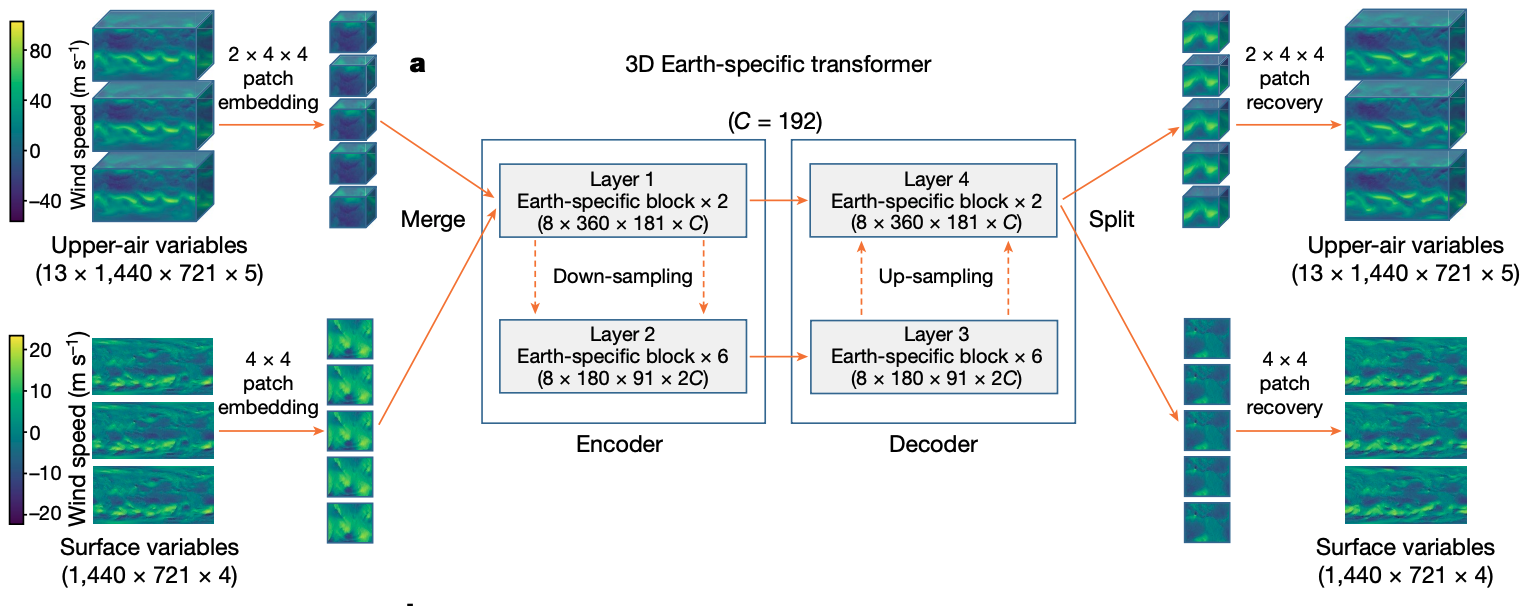
\includegraphics[width=\linewidth]{fig/pangu.png}}
		\caption{3DEST architecture.
		Based on the standard encoder–decoder design of vision transformers,
		we adjusted the shifted-window mechanism and applied an Earth-specific
		positional bias.\footnotemark}
\end{figure}
	\footnotetext{Bi, Kaifeng, et al. "Accurate medium-range global weather forecasting with 3D neural networks." Nature 619.7970 (2023): 533-538.}
\end{frame}

\begin{frame}{How to do long time prediction?}
	One of the bottleneck for ROM is the long time prediction accuracy: e.g. for weather forecasting,
	most data-driven models outperform numerical weather prediction over the 0-7 days regime but
	quickly 

	Several methods to perform time series prediction:
	\begin{itemize}
		\item * Hierarchical temporal aggregation
		\item * Manifold regularization
		\item * Nonlinear stability issue, especially compared with classical numerical stability
	\end{itemize}
\end{frame}

\begin{frame}{Operator inference ROM}
	Mesh-based $\Longrightarrow$ Mesh-free

	Another kind of nonlinear ROM is based on operator inference. A heuristic:
	Classical mesh-based solver amounts to solve the high dimesional mapping between the discretization on
	the huge mesh, e.g. $\mbR^{N\times N\times N} \rightarrow \mbR^{N\times N\times N}$, how about considering directly
	$\mbR^3 \rightarrow \mbR$, which is usually a nonlinear map\footnotemark.

	\textbf{Can be viewed as learning the reduced basis and operator simultaneously}
	\footnotetext{Mildenhall, Ben, et al. "Nerf: Representing scenes as neural radiance fields for view synthesis." Communications of the ACM 65.1 (2021): 99-106.
	}
\end{frame}

\begin{frame}{Operator inference ROM}
	More over, the parameter can also be fitted into this framework by encoding it as a latent vector\footnotemark
	\begin{figure}[ht]
		\centering
		\centerline{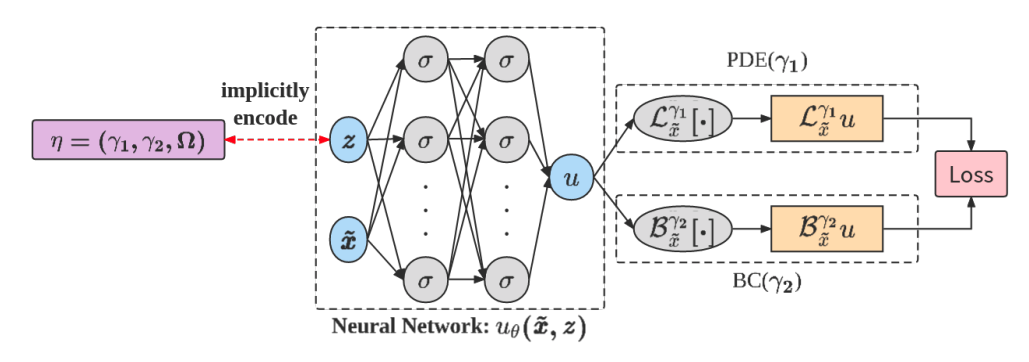
\includegraphics[width=\linewidth]{fig/MAD.png}}
		\caption{
		Architecture of Meta-Auto-Decoder..\footnotemark}
\end{figure}
	\footnotetext{Park, Jeong Joon, et al. "Deepsdf: Learning continuous signed distance functions for shape representation." Proceedings of the IEEE/CVF conference on computer vision and pattern recognition. 2019.
	}
\end{frame}

\begin{frame}{Relation to the sequence modeling}
	Given that present ROM are more and more similar to the sequence modeling in lots of CS application, i.e.
	non-intrusive method, similar transformer network. I personally think it worth to think carefully about their
	relationship.
	\begin{itemize}
		\item * Seq2Seq seems still not prevalent in scientific time series modeling.
		\item * Stability and out-of-distribution issue
	\end{itemize}
\end{frame}

\begin{frame}{Part II:}
	
\end{frame}

\begin{frame}
	Consider the parametrized PDE of the following form:
	\begin{equation*}
		\bm{F}(\mfu; \bm{\mu}) = 0.
	\end{equation*}

	A reduction operator $\mcA$ leads to the reduced field $\overline{\mfu}
	= \mcA(\mfu)$:. Then, the closure problem amounts to resolve the term
	\begin{equation*}
		\bm{C}(\bm{u}, \overline{\mfu}; \bm{\mu}) = \overline{\bm{F}}(\mfu; \bm{\mu}) -
		 \bm{F}(\overline{\mfu}; \bm{\mu})
	\end{equation*}
\end{frame}

\begin{frame}
	Caveat: in reduced order modeling, people are ``close the equation'' instead of 
	learning the closure model. This is different as closure model means that to
	increase the dimension of the descriptive variable so that with the closure
	variable the dynamics can be completely determined by the new state variable.
	While closing the equation just means to make sure there is no residue of the
	equation.
\end{frame}

\begin{frame}{Part III: A ``case'' study on collective variable (CV)\footnotemark}
	% TODO: this part is a bit wordy, try to simplify so that it looks clean.
	\begin{itemize}
		\item * Transfer operator framework
		\item * Effective dynamics
		\item * Algorithms
	\end{itemize}
	\footnotetext{Zhang, Wei, and Christof Schütte. "On finding optimal collective
	variables for complex systems by minimizing the deviation between effective and
	full dynamics." arXiv preprint arXiv:2405.02001 (2024).}
\end{frame}

\begin{frame}{Basic settings}
	Consider a stationary, ergodic, and discrete in time Markov chain $X_n \in \mbR^d$
	with transition probability $p(x, y)$ and invariant measure $\pi(dx)$. 

	The transfer operator associated with the dynamics is defined as 
	\begin{equation*}
		(\mcT f)(x) = \int_{\mbR^d} f(y)p(x, y)dy.
	\end{equation*}
	In deterministic dynamics, the transfer operator coincides with the Koopman operator.

	The Dirichlet form is defined as 
	\begin{equation*}
		\mcE(f, g)= \half \int_{\mbR^d}\int_{\mbR^d}p(x, y)(f(x) - f(y))
			(g(x) - g(y))\pi(x)dxdy.
	\end{equation*}

	If the dynamics is reversible, the transfer operator is self-adjoint and the
	Dirichlet form is symmetric.
\end{frame}

\begin{frame}{Spectrum and timescale}
	The spectrum of the transfer operator is related to the timescale of the dynamics
	and is an important quantity to be studied.
	\begin{theorem}
		If $p(x, y) > 0, \pi(x) > 0$, $\mcT$ is self-adjoint, and further
		\begin{equation*}
			\int_{\mbR^d}\int_{\mbR^d}p(x, y)p(y, x)dxdy < \infty,
		\end{equation*}
		Then, we have that $\mcT$ is a compact (Hilbert-Schmidt) operator whose non-zero spectrum
		are all eigenvalues. Moreover, any real eigenvalue belongs to $[-1, 1]$
		and the only eigenfunction of $\lambda = 1$ is the constant function.
	\end{theorem}
	This is the functional analysis generalization for the Perron-Frobenius theorem for
	stochastic matrices.
\end{frame}

\begin{frame}{Collective variable}
	A commonly adopted strategy is to utilize the fact that the dynamics of
	high-dimensional systems, e.g. molecular systems in MD and materials science,
	can often be well characterized using only a few observables, often called
	collective variables (CVs) or reaction coordinates, of the systems. For example,
	temperature, pressure, entropy, Gibbs free energy is used in the thermodynamical
	description of the ideal gas.

	CV can be viewed from the perspective of dimension reduction. PCA, one of the most
	important dimension reduction method, choose map from the first several singular
	(eigen-) vectors. So a primary choice is to chose CV as the eigenfunction of the
	transfer operator.
\end{frame}

\begin{frame}{Transfer operator eigenfunction}
	The eigenfunction of the transfer operator can be characterized by the following method:
	\begin{theorem}
		The solution of the following optimization problem
		\begin{equation*}
			\min_{f_1, ..., f_m} \sum_{i=1}^m \omega_i \mcE(f_i)
		\end{equation*}
		under the constraint that the basis $f_1, ..., f_m$ are orthognormal is given by
		the first $m$ eigenfunctions of the transfer operator.
	\end{theorem}
	However, it is hard to numerically solve this optimization problem if the dimension
	of the underlying space is high and to enforce the orthognormality constraint become
	hard to implement.
\end{frame}

\begin{frame}{Design the CV map: I}
	The Dirichlet form can be estimated according to the sample from the invariant
	distribution as:
	\begin{theorem}
		The CV map defined by the first eigenfunction of the transfer operator
		minimizes the averaged of quadratic variations:
		\begin{equation*}
			\min_f \mcE(f) \approx \min_f \lim_{N\rightarrow \infty}\frac{1}{2N}\sum_{n=0}^{2N-1}
			\norml f(X_{i+1}) - f(X_i) \normr_{\omega}^2,
		\end{equation*}
		among all the orthognormal basis $f$.
	\end{theorem}
	The weights $\omega$ are introduced in order to remove the non-uniqueness of
	the minimizer of due to permutation. \textbf{Interpretation: } $\xi$ should be a slow variable such that the observations $\xi(X_0), \xi(X_1), ...$
	vary slowly (in most of the time unless essential transitions occur) as the dynamics
	$X_n$ evolves.
\end{frame}

\begin{frame}{Transition rate}
	Commitor function is one of the well-known object to be studied in the rare event
	simulation. It is defined as
	\begin{equation}
		q(x) = \mcP(\text{starting from $x$, $X_n$ enters $B$ before it enters $A$.}).
	\end{equation}
	There is another quantity called the transition rate $k_{AB}$, which is formally
	defined as the ratio of the time spent in transition between $A$ and $B$ to the
	whole trajectory.
	\begin{theorem}
		Commitor function is the minimizer of the Dirichlet energy under the constraint that
		\begin{equation}
			f\big|_{A} = 0, \quad f\big|_{B} = 1.
		\end{equation}
		The minimum value is given by the transition rate $k_{AB}$.
	\end{theorem}
\end{frame}

\begin{frame}{Effective dynamics}
	Suppose we have a CV map $\xi: \mbR^d \rightarrow \mbR^k$, define the level set
	$\Sigma_z := \{ x\in\mbR^d, \xi(x) = z \}$. $\mu_z(dx) \in \mcP(\Sigma_z)$ is
	the conditional distribution given $z$. $\wtd \mu \in \mcP(\mbR^k)$ is the
	pushforward of the measure $\mu$ by $\xi$.
	\begin{definition}[Effective dynamics]
		The effective dynamics of $X_n$ associated to the CV map $\xi: \mbR^d
		\rightarrow \mbR^k$ is defined as the Markoc process $Z_n$ in $\mbR^k$
		with transition probability $\wtd p(z, \wht z)$:
		\begin{equation*}
			\begin{aligned}
				\wtd p(z, \wht z) = & \ \int_{\Sigma_z}\lb \int_{\mbR^d} p(x, y)\delta(\xi(y) - \wht z) dy \rb \mu_z(dx)		\\
				= & \ \frac{1}{Q(z)}\int_{\mbR^d}\int_{\mbR^d} p(x, y)\delta(\xi(x) - z) \delta(\xi(y) - \wht z) \pi(dx) dxdy.
			\end{aligned}
		\end{equation*}
	\end{definition}
\end{frame}

\begin{frame}{Variational characterization}
	The transition probability of the effective dynamics can be viewed as an
	approximation of the original dynamics in the following sense:
	\begin{equation*}
		\begin{aligned}
			p(x, y) &= p(\wht z | x)p(y | \wht z, x),		\\
			\overline{p}(x, y) &= p_{\theta}(\wht z | \xi(x))p_{\varphi}(y | \wht z),
		\end{aligned}
	\end{equation*}
	\begin{theorem}[Variational formulation]
		The minimizer of the following problem
		\begin{equation*}
			\arg\min_{\overline{p} \in \Theta^{\xi}}\mbE_{x\sim \mu} \lb\KL(p(x, \cdot)||\overline{p}(x, \cdot))\rb
		\end{equation*}
		is given by $p_{\theta} = \wtd p, p_{\varphi} = p_z$ where
		$p_z = \frac{d\mu_z}{d\sigma_{\Sigma_z}}$.
	\end{theorem}
\end{frame}

\begin{frame}{Design the CV map: II}
	\begin{theorem}
		Choose the CV map $\xi$ to minimize the KL divergence as
		\begin{equation*}
			\min_{\xi, \overline{p} \in \Theta^{\xi}} \mbE_{x\sim \mu} \lb\KL(p(x, \cdot)||\overline{p}(x, \cdot))\rb
		\end{equation*}
	\end{theorem}

	Personal comment: this is somehow similar to the latent variable generative model
	such as VAE with ELBO loss.

	It would also be inspiring to work out a toy case where we can exactly identify the
	minimizer of the problem, e.g. $\mu$ is Gaussian.
\end{frame}

\begin{frame}{Error estimate}
	\begin{theorem}[Transition rates]
		Assume that the sets $A, B \subset \mbR^d$ are related to the sets
		$\wtd A, \wtd B \subset \mbR^k$ throught the CV map $\xi$ via
		$A = \xi^{-1}(\wtd A), B = \xi^{-1}(\wtd B)$. Let $q, k_{AB}$ denote the
		commitor and the transition rate of $X_n$ from $A$ to $B$ respectively.
		\begin{equation*}
			\wtd k_{\wtd A\wtd B} = k_{AB} + \mcE(q - \wtd q \circ \xi).
		\end{equation*}
	\end{theorem}
\end{frame}

\begin{frame}{How should define a good CV?}
	\begin{itemize}
		\item Do we really need to achieve a low reconstruction error or a low KL-divergence
		for a good CV? The answer is not clear. For example, as a CV, the commitor function
		distinguishs between two attractor basin even if it is only an one-dimensional CV.
		\item How can we characterize the classical CV such as the pressure, temperature,
		entropy, etc. Are they really minimizing the reconstruction error or the KL-divergence?
		\item Another approach is to start from one well-known CV such as density for the study
		of water and trying to ask what will be a good extra CV to be used together with the
		water.
	\end{itemize}
\end{frame}

\end{document}